%iffalse%\let\negmedspace\undefined
\let\negthickspace\undefined
\documentclass[journal,12pt,onecolumn]{IEEEtran}
\usepackage{cite}
\usepackage{amsmath,amssymb,amsfonts,amsthm}
\usepackage{algorithmic}
\usepackage{graphicx}
\usepackage{textcomp}
\usepackage{xcolor}
\usepackage{txfonts}
\usepackage{listings}
\usepackage{enumitem}
\usepackage{mathtools}
\usepackage{gensymb}
\usepackage{comment}
\usepackage[breaklinks=true]{hyperref}
\usepackage{tkz-euclide} 
\usepackage{listings}
\usepackage{gvv}                                        
%\def\inputGnumericTable{}                                 
\usepackage[latin1]{inputenc}     
\usepackage{xparse}
\usepackage{color}                                            
\usepackage{array}                                            
\usepackage{longtable}                                       
\usepackage{calc}                                             
\usepackage{multirow}
\usepackage{multicol}
\usepackage{hhline}                                           
\usepackage{ifthen}                                           
\usepackage{lscape}
\usepackage{tabularx}
\usepackage{array}
\usepackage{float}
\newtheorem{theorem}{Theorem}[section]
\newtheorem{problem}{Problem}
\newtheorem{proposition}{Proposition}[section]
\newtheorem{lemma}{Lemma}[section]
\newtheorem{corollary}[theorem]{Corollary}
\newtheorem{example}{Example}[section]
\newtheorem{definition}[problem]{Definition}
\newcommand{\BEQA}{\begin{eqnarray}}
\newcommand{\EEQA}{\end{eqnarray}}
\usepackage{float}
%\newcommand{\define}{\stackrel{\triangle}{=}}
\theoremstyle{remark}
\usepackage{ circuitikz }
%\newtheorem{rem}{Remark}
% Marks the beginning of the document this one


\begin{document}
\title{
ASSIGNMENT 5: GATE 2020 MINING ENGINEERING  }\\

\author{AI25BTECH11039 - Harichandana Varanasi }
\maketitle
\renewcommand{\thefigure}{\theenumi}
\renewcommand{\thetable}{\theenumi}

\begin{enumerate}

\item The eigenvalues of the matrix $A=\myvec{1 & 4 \\ 3 & 2}$ are

\hfill{\brak{\text{GATE MN 2020}}}

\begin{enumerate}
\begin{multicols}{2}
\item $6,4$
\item $4,5$
\item $-2,5$
\item $-4,5$
\end{multicols}
\end{enumerate}

\item For the electric delay detonator shown in the figure, the components P, Q and R, respectively, are

\hfill{\brak{\text{GATE MN 2020}}}

\begin{figure}[H]
\centering
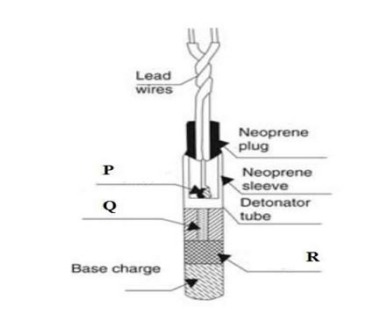
\includegraphics[width=0.3\columnwidth]{figs/2018MN2.jpeg}
\caption*{}
\label{fig:q2}
\end{figure}

\begin{enumerate}
\item fuse head, delay element, priming charge
\item fuse head, priming charge, delay element
\item priming charge, delay element, fuse head
\item delay element, fuse head, priming charge
\end{enumerate}

\item Match the following safety arrangements for a surface-to-underground shaft hoist with their corresponding safety functions.
\begin{center}
\begin{tabular}{ll}
\textbf{Hoisting safety arrangement} & \textbf{Safety function} \\
P. Detaching hook & 1. Over-winding safety on surface \\
Q. Narrowing rigid guides & 2. Resting cages \\
R. Keps & 3. Over-winding safety at underground \\
\end{tabular}
\end{center}

\hfill{\brak{\text{GATE MN 2020}}}

\begin{enumerate}
\begin{multicols}{2}
\item P-1, Q-2, R-3
\item P-3, Q-1, R-2
\item P-2, Q-3, R-1
\item P-1, Q-3, R-2
\end{multicols}
\end{enumerate}

\item The fore bearings and back bearings of the lines of an open compass traverse are given below.
\begin{center}
\begin{tabular}{|l|l|l|}
\hline
\textbf{Line} & \textbf{Fore bearing} & \textbf{Back bearing} \\ \hline
PQ & $132^{\circ}30^{\prime}$ & $313^{\circ}30^{\prime}$ \\ \hline
QR & $123^{\circ}30^{\prime}$ & $303^{\circ}30^{\prime}$ \\ \hline
RS & $182^{\circ}30^{\prime}$ & $2^{\circ}15^{\prime}$ \\ \hline
ST & $288^{\circ}45^{\prime}$ & $108^{\circ}0^{\prime}$ \\ \hline
\end{tabular}
\end{center}
The stations that are free from local attraction are

\hfill{\brak{\text{GATE MN 2020}}}

\begin{enumerate}
\begin{multicols}{2}
\item P and Q
\item Q and R
\item R and S
\item S and T
\end{multicols}
\end{enumerate}

\item The plane stress condition is given by

\hfill{\brak{\text{GATE MN 2020}}}

\begin{enumerate}
\begin{multicols}{2}
\item $\epsilon_{zz}=0, \gamma_{yz}=0, \gamma_{zx}=0$
\item $\sigma_{zz}=0, \tau_{yz}=0, \tau_{zx}=0$
\item $\sigma_{zz}\ne0, \tau_{yz} \ne 0, \tau_{zx}\ne0$
\item $\epsilon_{zz}\ne0, \gamma_{yz}\ne0, \gamma_{zx}\ne0$
\end{multicols}
\end{enumerate}

\item Match the following metals with their corresponding minerals.
\begin{center}
\begin{tabular}{ll}
\textbf{Metal} & \textbf{Mineral} \\
P. Copper & 1. Galena \\
Q. Tungsten & 2. Sphalerite \\
R. Lead & 3. Chalcopyrite \\
S. Zinc & 4. Wolframite \\
\end{tabular}
\end{center}

\hfill{\brak{\text{GATE MN 2020}}}

\begin{enumerate}
\begin{multicols}{2}
\item P-4, Q-2, R-1, S-3
\item P-4, Q-1, R-3, S-2
\item P-3, Q-4, R-1, S-2
\item P-2, Q-3, R-4, S-1
\end{multicols}
\end{enumerate}

\item Match the wire rope types with their corresponding cross-sectional diagrams.

\begin{figure}[H]
\centering
\caption*{}
\label{fig:q7}
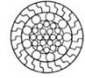
\includegraphics[width=0.2\columnwidth]{figs/2020mn7a.jpeg}
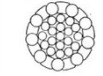
\includegraphics[width=0.2\columnwidth]{figs/2020mn7b.jpeg}
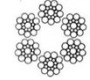
\includegraphics[width=0.2\columnwidth]{figs/2020mn7c.jpeg}
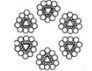
\includegraphics[width=0.2\columnwidth]{figs/2020mn7d.jpeg}
\end{figure}
\begin{center}
\begin{tabular}{ll}
\textbf{Rope type} & \textbf{Diagrams} \\
P. Round strand & 1. \\
Q. Half-locked coil & 2. \\
R. Flattened strand & 3. \\
S. Full locked coil & 4. \\
\end{tabular}
\end{center}

\hfill{\brak{\text{GATE MN 2020}}}

\begin{enumerate}
\begin{multicols}{2}
\item P-3, Q-2, R-4, S-1
\item P-3, Q-1, R-2, S-4
\item P-1, Q-3, R-4, S-2
\item P-4, Q-2, R-3, S-1
\end{multicols}
\end{enumerate}

\item The 'ratchet and pawl mechanism' in a jack hammer drill

\hfill{\brak{\text{GATE MN 2020}}}

\begin{enumerate}
\item forces down the piston
\item provides a twisting force to the drill steel
\item engages rifle bar with rifle nut
\item prevents reverse rotation of rifle bar
\end{enumerate}

\item Post-pillar method of stoping is a variant of

\hfill{\brak{\text{GATE MN 2020}}}

\begin{enumerate}
\begin{multicols}{2}
\item cut and fill stoping
\item sublevel stoping
\item vertical crater retreat method
\item sublevel caving
\end{multicols}
\end{enumerate}

\item Cross-measure borehole method is used for

\hfill{\brak{\text{GATE MN 2020}}}

\begin{enumerate}
\begin{multicols}{2}
\item rock slope monitoring
\item methane drainage
\item connecting two drifts
\item subsidence monitoring
\end{multicols}
\end{enumerate}

\item The dry and wet bulb temperatures at the inlet of the airstream are $30^{\circ}$C and $25^{\circ}$C respectively. The corresponding values at the outlet of the airstream are $26^{\circ}$C and $25^{\circ}$C respectively. The psychrometric process that occurs in the airstream is described as

\hfill{\brak{\text{GATE MN 2020}}}

\begin{enumerate}
\begin{multicols}{2}
\item latent cooling
\item sensible cooling
\item condensation
\item evaporative cooling
\end{multicols}
\end{enumerate}

\item For a mixture of inflammable gases, the lower and upper explosibility limits can be computed using

\hfill{\brak{\text{GATE MN 2020}}}

\begin{enumerate}
\begin{multicols}{2}
\item Dalton's law
\item Graham's law
\item Le Chatelier relation
\item Boyle's law
\end{multicols}
\end{enumerate}

\item The code for the lowest category of mineral resources under United Nations Framework Classification \brak{UNFC} system is

\hfill{\brak{\text{GATE MN 2020}}}

\begin{enumerate}
\begin{multicols}{2}
\item $444$
\item $123$
\item $334$
\item $111$
\end{multicols}
\end{enumerate}

\item Match the following sampling patterns with the corresponding sampling types.

\begin{figure}[H]
\centering
\caption*{}
\label{fig:q14}
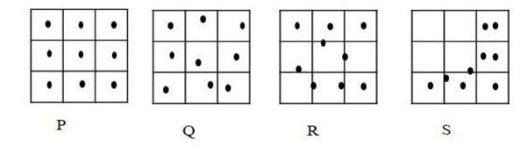
\includegraphics[width=0.5\columnwidth]{figs/2020mn14.jpeg}

\end{figure}
\begin{center}
\begin{tabular}{ll}
\textbf{Sampling Pattern} & \textbf{Sampling Type} \\
P. & 1. Regular \\
Q. & 2. Biased \\
R. & 3. Stratified random \\
S. & 4. Random \\
\end{tabular}
\end{center}

\hfill{\brak{\text{GATE MN 2020}}}

\begin{enumerate}
\begin{multicols}{2}
\item P-1, Q-3, R-2, S-4
\item P-1, Q-3, R-4, S-2
\item P-1, Q-2, R-3, S-4
\item P-4, Q-2, R-1, S-3
\end{multicols}
\end{enumerate}

\item In the context of gas testing using flame safety lamp, the correct statement is

\hfill{\brak{\text{GATE MN 2020}}}

\begin{enumerate}
\item Each accumulation test has to be necessarily followed by percentage test
\item Accumulation test is always done after percentage test
\item Either percentage test or accumulation test can be done first
\item Percentage test is done only in the event of accumulation test giving negative result
\end{enumerate}

\item For x in the range of [-3, 3], the maximum value for the function $f(x)=x^{3}-6x^{2}+9x+15$ is \underline{\hspace{2cm}} \brak{\text{round off to 1 decimal place}}.

\hfill{\brak{\text{GATE MN 2020}}}

\item A rock sample has coefficient of thermal diffusivity $1.282\times10^{-6}m^{2}/s$, specific heat $900 J/\brak{kg^{\circ}C}$ and density $2600~kg/m^{3}.$ The coefficient of thermal conductivity of the rock sample in $W/\brak{m^{\circ}C}$ is \underline{\hspace{2cm}} \brak{\text{round off to 1 decimal place}}.

\hfill{\brak{\text{GATE MN 2020}}}

\item A random variable X has the following probability mass function.
\begin{center}
\begin{tabular}{|l|l|l|l|l|}
\hline
X & 3 & 6 & 8 & 12 \\ \hline
f(x) & $1/2$ & $1/4$ & $1/8$ & $1/8$ \\ \hline
\end{tabular}
\end{center}
The expected value of the variable X is \underline{\hspace{2cm}} \brak{\text{round off to 1 decimal place}}.

\hfill{\brak{\text{GATE MN 2020}}}

\item A random sample has five observations as shown below.
$11, 12, 14, 15, 13$
The coefficient of variation of the sample is \underline{\hspace{2cm}} \brak{\text{round off to 3 decimal places}}.

\hfill{\brak{\text{GATE MN 2020}}}

\item Rock strata has unit weight of $25 kN/m^{3}$ and Poisson's ratio $1/3$. At a depth of 200 m, the horizontal stress in MPa is \underline{\hspace{2cm}} \brak{\text{round off to 1 decimal place}}.

\hfill{\brak{\text{GATE MN 2020}}}

\item A shovel of bucket capacity $4.2~m^{3}$ makes 900 passes per day with a fill factor of 0.8. If the swell factor of the rock is 1.4, then in-situ volume handled by the shovel in a month of 24 working days in $m^{3}$ is \underline{\hspace{2cm}} \brak{\text{round off to 1 decimal place}}.

\hfill{\brak{\text{GATE MN 2020}}}

\item A cylindrical sample of granular material has the following measurements:
Length: 10 cm
Diameter: 5 cm
Weight: 350 g
Assume the sample is completely dry with specific gravity of solid grains 2.8. The void ratio of the sample is \underline{\hspace{2cm}} \brak{\text{round off to 3 decimal places}}.

\hfill{\brak{\text{GATE MN 2020}}}

\item The following consecutive readings were taken at uniform intervals with a level and a levelling staff on continuously sloping ground.
$0.405, 1.035, 1.654, 0.240, 0.615, 1.125, 0.800, 1.125$
The number of change points is \underline{\hspace{2cm}}.

\hfill{\brak{\text{GATE MN 2020}}}

\item The cost of a slurry pump is Rs. 50,000 and it has an estimated life of 7 years. If the salvage value is Rs. 8,000, the annual depreciation following straight-line depreciation method, in Rupees, is \underline{\hspace{2cm}} \brak{\text{round off to 1 decimal place}}.

\hfill{\brak{\text{GATE MN 2020}}}

\item In a mine bench, the shovel loading time follows exponential distribution with a mean loading time of 5 min per dumper. The arrival rate of dumpers that are identical in capacity, follows Poisson distribution with a mean arrival rate of 8 per hour. The probability that the shovel remains idle is \underline{\hspace{2cm}} \brak{\text{round off to 2 decimal places}}.

\hfill{\brak{\text{GATE MN 2020}}}

\item For $w=\frac{e^{t}-t}{e^{t}+t}$, the value of $\frac{dw}{dt}$ is

\hfill{\brak{\text{GATE MN 2020}}}

\begin{enumerate}
\begin{multicols}{2}
\item $\frac{2e^{t}\brak{t^{2}+1}}{\brak{e^{t}-t^{2}}^{2}}$
\item $\frac{2e^{t}\brak{t-1}}{\brak{e^{t}+t}^{2}}$
\item $\frac{2e^{t}\brak{t^{2}-1}}{\brak{e^{t}+t^{2}}^{2}}$
\item $\frac{2e^{t}\brak{t+1}}{\brak{e^{t}-t}^{2}}$
\end{multicols}
\end{enumerate}

\item For the differential equation $y\sqrt{1-x^{2}}dy+x\sqrt{1-y^{2}}dx=0$, assuming the constant of integration to be C, the general solution is

\hfill{\brak{\text{GATE MN 2020}}}

\begin{enumerate}
\begin{multicols}{2}
\item $\frac{1}{\sqrt{1-x^{2}}}+\frac{1}{\sqrt{1-y^{2}}}=C$
\item $y\sqrt{1-x^{2}}+x\sqrt{1-y^{2}}=C$
\item $\sqrt{1-x}+\sqrt{1-y}=C$
\item $\sqrt{1-x^{2}}+\sqrt{1-y^{2}}=C$
\end{multicols}
\end{enumerate}

\item A belt-drive used for power transmission between two parallel shafts has a belt of mass $1.2~kg/m$, and the maximum allowable belt tension is 2250 N. If the centrifugal tension is one third of the maximum allowable belt tension, the speed at which maximum power is transmitted by the belt, in $m/s$, is

\hfill{\brak{\text{GATE MN 2020}}}

\begin{enumerate}
\begin{multicols}{2}
\item $46.48$
\item $38.73$
\item $25.00$
\item $35.36$
\end{multicols}
\end{enumerate}

\item An air receiver of a compressor, having volume $0.5~m^{3},$ supplies air for charging ANFO in drill holes. During the charging process the absolute pressure of the air receiver falls from 900 kPa to 700 kPa. Assuming the entire process is isothermal, the volume of air supplied by the receiver at 100 kPa ambient pressure, in $m^{3}$ is

\hfill{\brak{\text{GATE MN 2020}}}

\begin{enumerate}
\begin{multicols}{2}
\item $1.00$
\item $0.39$
\item $0.64$
\item $4.48$
\end{multicols}
\end{enumerate}

\item A conveyor belt consumes 60 kW power while running at a speed of $3.0~m/s$. The angle of lap is $180^{\circ}$ and the coefficient of friction between belt and pulley is 0.2. The maximum tension \brak{kN} in the belt is

\hfill{\brak{\text{GATE MN 2020}}}

\begin{enumerate}
\begin{multicols}{2}
\item $21.7$
\item $61.7$
\item $82.9$
\item $42.9$
\end{multicols}
\end{enumerate}

\item A linear programming problem is stated below.
Maximize $Z=3x_{1}+5x_{2}$
subject to, $2x_{1}+x_{2}\le8$
$6x_{1}+8x_{2}\le30$
$x_1, x_{2}\ge0$
The objective function has

\hfill{\brak{\text{GATE MN 2020}}}

\begin{enumerate}
\begin{multicols}{2}
\item infinite number of solutions
\item unbounded solution
\item unique solution
\item infeasible solution
\end{multicols}
\end{enumerate}

\item An explosive mixture has 80 g of ammonium nitrate \brak{NH4NO3} and 14 g of fuel oil \brak{$C_{10}H_{20}$}. The oxygen balance in the mixture is

\hfill{\brak{\text{GATE MN 2020}}}

\begin{enumerate}
\begin{multicols}{2}
\item surplus by 32 g
\item deficient by 24 g
\item surplus by 16 g
\item deficient by 32 g
\end{multicols}
\end{enumerate}

\item A cylindrical sample of cross-sectional area A, length L, and Young's Modulus E, is subjected to a constant uniaxial load P. Within the elastic limit of loading, the total strain energy stored is

\hfill{\brak{\text{GATE MN 2020}}}

\begin{enumerate}
\begin{multicols}{2}
\item $\frac{2P^{2}L}{AE}$
\item $\frac{P^{2}L}{2AE}$
\item $\frac{PL}{A^{2}E}$
\item $\frac{P^{2}L}{AE}$
\end{multicols}
\end{enumerate}

\item A surface mine production system along with the reliability of the individual components is shown below. The system reliability is \underline{\hspace{2cm}} \brak{\text{round off to 3 decimal places}}.

\hfill{\brak{\text{GATE MN 2020}}}

\begin{figure}[H]
\centering
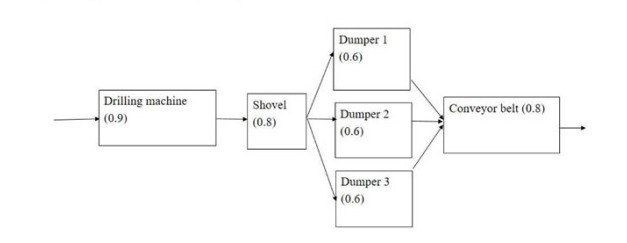
\includegraphics[width=0.9\columnwidth]{figs/2020mn34.jpeg}
\caption*{}
\label{fig:q34}
\end{figure}

\item The selling price of one rock bolt \brak{in Rs.} is given as, $S=\brak{200-10n^{-0.5}}$ where n is the number of bolts produced. The manufacturing cost of rock bolts has a fixed component of Rs. 15000, and a variable component of Rs. 100 per bolt. The minimum break-even production, in number of rock bolts, is \underline{\hspace{2cm}} \brak{\text{round off to 1 decimal place}}.

\hfill{\brak{\text{GATE MN 2020}}}

\item Two underground mines are separated by a horizontal coal barrier of 60 m thickness. One mine is inundated, whereas the other mine has a blind heading of dimensions 4.0 m wide and 2.5 m height terminating at the barrier. The overall in-situ shear strength of the coal mass is 500 kPa. Assume that the failure mode is in shear. At a factor of safety of 10, the maximum water head that can be withstood by the coal barrier, in m, is \underline{\hspace{2cm}} \brak{\text{round off to 1 decimal place}}.

\hfill{\brak{\text{GATE MN 2020}}}

\item Air enters from ambient atmosphere into a level duct of uniform cross-section area $0.2~m^{2}$ at a flow rate of $2.0~m^{3}/s$ and density of $1.2~kg/m^{3}$. The entry shock loss factor is 1.0 and the resistance of the duct per meter length is $1.0~Ns^{2}/m^{8}$. The static pressure measured at a distance of 20 m from the duct entrance in Pa, is \underline{\hspace{2cm}} \brak{\text{round off to 1 decimal place}}.

\hfill{\brak{\text{GATE MN 2020}}}

\item A sealed-off area air sample consists of 16.0\% $O_{2}$, 3.0\% $CO_{2}$ and the rest is $N_{2}$. Assume that the standard composition of atmospheric air is 21.0\% $O_{2}$ and 79.0\% $N_{2}$. The percentage of blackdamp in the air sample is \underline{\hspace{2cm}} \brak{\text{round off to 2 decimal places}}.

\hfill{\brak{\text{GATE MN 2020}}}

\item A diesel loader produces 60 $l/s$ of exhaust fumes containing 5000 ppm of CO. The incoming air has 10 ppm of CO. The minimum amount of air flow in $m^{3}/s$ that is needed at the loader to dilute CO to a permissible level of 50 ppm is \underline{\hspace{2cm}} \brak{\text{round off to 1 decimal place}}.

\hfill{\brak{\text{GATE MN 2020}}}

\item The equation for peak particle velocity \brak{PPV} from blast induced ground vibration is given by
$PPV=k\brak{\frac{D}{\sqrt{Q}}}^{B}$.
where k and B are site constants.
In a field study, the following readings are recorded.
\begin{center}
\begin{tabular}{|p{1.5cm}|p{1.5cm}|p{3cm}|p{2cm}|}
\hline
\textbf{Sensor No.} & \textbf{PPV in $mm/s$} & \textbf{Sensor distance from blast site \brak{D} in m} & \textbf{Charge per delay \brak{Q} in kg} \\ \hline
1 & 5.5 & 200 & 100 \\ \hline
2 & 3.4 & 300 & 100 \\ \hline
\end{tabular}
\end{center}
The value of B is \underline{\hspace{2cm}} \brak{\text{round off to 3 decimal places}}.

\hfill{\brak{\text{GATE MN 2020}}}

\item An underground copper mine sends 2500 tonnes of ore per day to the concentrator plant having an average grade of 1.2\% Cu. The plant produces concentrate of 25.0\% Cu with a recovery of 93.0\%. The solids portion of tailings generated from the plant per day in tonnes is \underline{\hspace{2cm}} \brak{\text{round off to 1 decimal place}}.

\hfill{\brak{\text{GATE MN 2020}}}

\item A mine gallery is supported by regularly placed roof bolts of 100 kN allowable pull force per bolt, as shown below. Assuming unit weight of the immediate roof is $25 kN /m^{3}$, the factor of safety of the support system is \underline{\hspace{2cm}} \brak{\text{round off to 2 decimal places}}.

\hfill{\brak{\text{GATE MN 2020}}}

\begin{figure}[H]
\centering
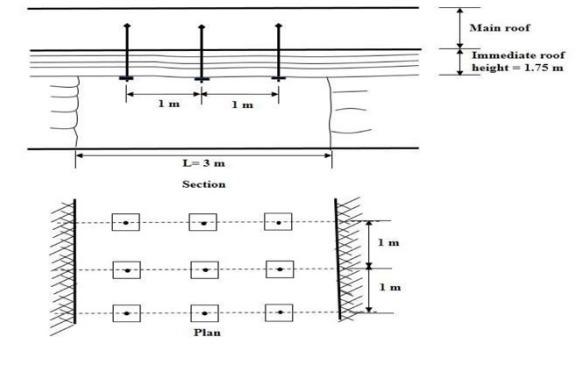
\includegraphics[width=0.8\columnwidth]{figs/2020mn42.jpeg}
\caption*{}
\label{fig:q42}
\end{figure}

\item The slip circle of radius 30.0 m in an overburden slope is shown with the centre of slip circle at point O. The tension crack is completely filled with water. For one meter width of the slope, the moment exerted by the force of water about O in kN-m is \underline{\hspace{2cm}} \brak{\text{round off to 1 decimal place}}.

\hfill{\brak{\text{GATE MN 2020}}}

\begin{figure}[H]
\centering
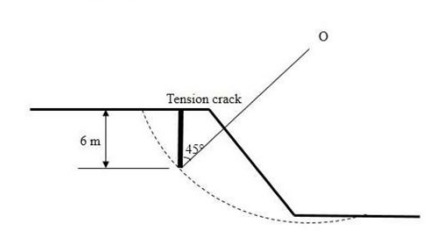
\includegraphics[width=0.7\columnwidth]{figs/2020mn43.jpeg}
\caption*{}
\label{fig:q43}
\end{figure}

\item The function values at four points of x are shown in the table. The area under the function, using trapezoidal method, is \underline{\hspace{2cm}} \brak{\text{round off to 1 decimal place}}.
\begin{center}
\begin{tabular}{|l|l|l|l|l|}
\hline
\textbf{X} & \textbf{2} & \textbf{4} & \textbf{8} & \textbf{9} \\ \hline
\textbf{f(x)} & 8 & 12 & 9 & 10 \\ \hline
\end{tabular}
\end{center}

\hfill{\brak{\text{GATE MN 2020}}}

\item A particle starting from rest moves in a straight line such that after time, t \brak{seconds}, the acceleration becomes $\brak{6-t/4}cm/s^{2}$. When the acceleration becomes zero, the velocity of the particle in cm/s is \underline{\hspace{2cm}} \brak{\text{round off to 1 decimal place}}.

\hfill{\brak{\text{GATE MN 2020}}}

\item A parallelepiped has edge vectors as shown below.
$\vec{A}=-4\hat{i}-10\hat{j}-\hat{k}$
$\vec{B}=7i+9j-2\hat{k}$
$\vec{C}=3\hat{i}+9\hat{j}+4\hat{k}$
The volume of the parallelepiped is \underline{\hspace{2cm}} \brak{\text{round off to 1 decimal place}}.

\hfill{\brak{\text{GATE MN 2020}}}

\item For a development heading, the blasting parameters are
Cross-section: $6.0~m\times5.0$ m
Total number of holes: 72
Number of trimmer holes: 30
Depth of each hole: 3.5 m
Charge per hole \brak{except trimmers}: 3.5 kg
Charge per trimmer hole: 1.8 kg
Pull per round: 90\% of hole depth
The powder factor for the development round in $m^{3}/kg$ is \underline{\hspace{2cm}} \brak{\text{round off to 2 decimal places}}.

\hfill{\brak{\text{GATE MN 2020}}}

\item The following figure represents the observations from the level survey of an underground gallery.
If the reduced level of station A is 100.0 m, the reduced level of station D in m is \underline{\hspace{2cm}} \brak{\text{round off to 1 decimal place}}.

\hfill{\brak{\text{GATE MN 2020}}}

\begin{figure}[H]
\centering
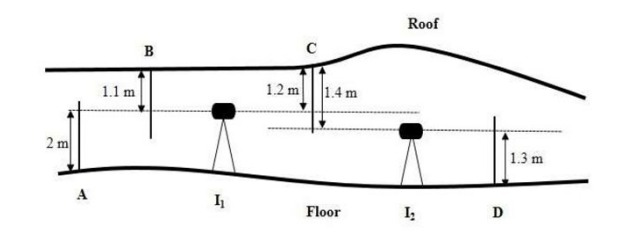
\includegraphics[width=0.9\columnwidth]{figs/2020mn48.jpeg}
\caption*{}
\label{fig:q48}
\end{figure}

\item A tacheometer was setup at station P and the following readings were taken at two stations A and B with the staff held vertical and the line of sight horizontal.
\begin{center}
\begin{tabular}{|l|l|l|}
\hline
\textbf{Line} & \textbf{Bearing} & \textbf{Staff intercept} \\ \hline
PA & $210^{\circ}$ & 1.2 m \\ \hline
PB & $135^{\circ}$ & 1.4 m \\ \hline
\end{tabular}
\end{center}
The additive and multiplying constants of the tacheometer are 0 and 100, respectively.
The length of AB in m is \underline{\hspace{2cm}} \brak{\text{round off to 1 decimal place}}.

\hfill{\brak{\text{GATE MN 2020}}}

\item The geometry of a simple planar curve \brak{ADB} is shown below. The value of the mid-ordinate of the curve in m is \underline{\hspace{2cm}} \brak{\text{round off to 1 decimal place}}.

\hfill{\brak{\text{GATE MN 2020}}}

\begin{figure}[H]
\centering
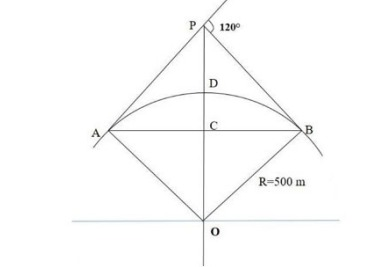
\includegraphics[width=0.6\columnwidth]{figs/2020mn50.jpeg}
\caption*{}
\label{fig:q50}
\end{figure}

\item A steel cube of side 50 mm is subjected to a uniform pressure of 200 MPa acting on each face. The Young's modulus and Poisson's ratio of the material are 200 GPa and 0.25, respectively. The decrease in the side of the cube in mm is \underline{\hspace{2cm}} \brak{\text{round off to 3 decimal places}}.

\hfill{\brak{\text{GATE MN 2020}}}

\item In the figure shown below, the friction coefficient between the block and the inclined plane is 0.2, and all the pulleys are weightless. The weight of the block is 10 N. The minimum force P in Newtons that is needed to slide the block up the inclined plane is \underline{\hspace{2cm}} \brak{\text{round off to 2 decimal places}}.


\hfill{\brak{\text{GATE MN 2020}}}

\begin{figure}[H]
\centering
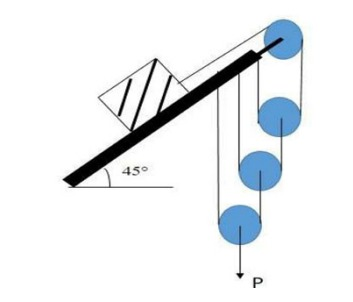
\includegraphics[width=0.5\columnwidth]{figs/2020mn52.jpeg}
\caption*{}
\label{fig:q52}
\end{figure}

\item An assignment problem is given below with the cost of assignment as shown.

If only one task can be assigned to one group, the minimum cost of assignment is \underline{\hspace{2cm}}.
\begin{center}
\begin{tabular}{|l|l|l|l|l|}
\hline
\textbf{Task} & \textbf{T1} & \textbf{T2} & \textbf{T3} & \textbf{T4} \\ \hline
\textbf{Group} & & & & \\ \hline
G1 & 6 & 10 & 5 & 4 \\ \hline
G2 & 4 & 100 & 6 & 4 \\ \hline
G3 & 6 & 9 & 6 & 2 \\ \hline
G4 & 3 & 7 & 6 & 4 \\ \hline
\end{tabular}
\end{center}

\hfill{\brak{\text{GATE MN 2020}}}

\item A vertical stoping block of length 60.0 m, height 40.0 m, and average width 1.5 m has sharp boundary walls. However, the mining width of the stoping block is 2.0 m. The tonnage factors are $3.0~tonne/m^{3}$ for ore and $2.5~tonne/m^{3}$ for wall rocks. The average grade of ore is 10.0\%. The overall grade of ore mined on account of dilution in percentage is \underline{\hspace{2cm}} \brak{\text{round off to 2 decimal places}}.

\hfill{\brak{\text{GATE MN 2020}}}

\item A bauxite ore body has four boreholes as shown below. For each borehole, the grade of alumina, the thickness of the ore body, and the triangular area of influence are as shown.
The average grade of ore body in the region ABCD in percentage is \underline{\hspace{2cm}} \brak{\text{round off to 1 decimal place}}.

\hfill{\brak{\text{GATE MN 2020}}}

\begin{figure}[H]
\centering
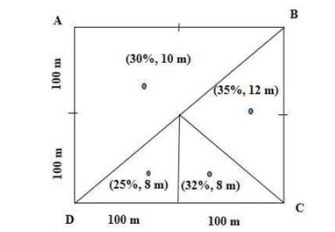
\includegraphics[width=0.7\columnwidth]{figs/2020mn55.jpeg}
\caption*{}
\label{fig:q55}
\end{figure}

\end{enumerate}

\end{document}
